\documentclass[12pt]{article}
\usepackage[a4paper, margin=1in]{geometry}
\usepackage{lmodern}
\usepackage{graphicx} % Required for inserting images
\usepackage{ucs}
\usepackage{notoccite}
\usepackage{float}
\usepackage{svg}
\svgsetup{inkscapeexe=inkscape}
\svgpath{{./Images/}}  % Set the path for SVGs
\usepackage{amsmath}
\usepackage{hyperref} % For clickable links
\graphicspath{{./Images/}}

\hypersetup{
    colorlinks=true,       % false: boxed links; true: colored links
    linkcolor=blue,        % color of internal links
    citecolor=blue,        % color of links to bibliography
    filecolor=magenta,     % color of file links
    urlcolor=cyan          % color of external links
}


\begin{document}


\section{VA001}
VA001 is a Basic self bias Miller Operational transcondutance amplifier, exemplified in Fig. \ref{VA001}.


%O start up esta mau, tem de ser alterado
\begin{figure}[H]
        \centering
        \includesvg[width=1\textwidth]{VA001.svg}
        \caption{proposed self bias two stage operational transcondutance amplifier.}
        \label{VA001}
\end{figure}
\subsection{Circuit explanation}
$P_1 - P_2$, $N_1 - N_4$, and $R_1$ form the biasing cell, functioning as a PTAT current bias generator.  

The proportional relationship comes from $N_3$ having a transconductance four times lower than that of $N_4$. As temperature increases, $V_{GS_3}$ rises, which increases the current through $N_4$ due to its higher transconductance, as both gates are connected. The current mirrors formed by $P_1$ and $P_2$ ensure equal currents, establishing an internal feedback loop. Transistors $N_1$ and $N_2$ limit the voltage across $N_3$ and $N_4$, thereby improving the PSRR. Additionally, $R_1$ introduces degeneration in $N_4$, allowing for better control over the reference current and transconductance.

To maximize PSRR and minimize unwanted feedback from the amplifier to the bias cell, the transistor sizes should not be excessively large, but minimum size transistors should be avoided at all cost, transistor with L or W close to the minimum size have a current curve with very prominent short channel effects that can impact a circuit very negatively, suffer more from hot carrier degradation and are very susceptible to random variation during fabrication. 


By assuming an initial condition of $V_{IN+} = V_{IN-} = V_{DD}/2$ every node in the circuit is fixed at some DC voltage value.  theoretical its assumed that $V_{OUT}=V_{DD}/2$ in this condition.
Focusing on the first stage, a change in $V_{IN+}$ equal to $\Delta V_{IN+}$ occurs leading to a symmetric current change of $-\Delta I_{PAIR+} = \Delta I_{PAIR-}$. This current change is expressed as $-\Delta I_{PAIR+} = \Delta V_{IN+} \times g_{mP6}$. Ignoring the current source $P_5$, the output variation of the first stage can be described as $-\Delta V_{IN+} \times g_{mP5} (R_{oP5} \parallel R_{oN6})$, where $g_{mP5} = g_{mP6}$ and the small-signal output impedance is the parallel combination of the output impedance's of $P_6$ and $N_6$.




Since $N_5$ is diode-connected, the current variation $\Delta I_{PAIR-}$ causes a corresponding $\Delta V_{GS_{N5}}$, which is proportional to $\Delta V_{IN+} \times g_{mP5}  \times R_{oN5}$.  Because $N_6$ shares the same gate potential, its output impedance inversely varies with $\Delta V_{IN+}$,  leading to a gain variation with $\Delta V_{IN+}$. While this typically poses no issue in a closed-loop configuration and a relatively small signal amplification, where the gain is stabilized by feedback, this variation introduces significant distortion in the output signal in open-loop configurations.


Since \( V_{\text{DS}_{N6}} = V_{\text{GS}_{N8}} \), any variation at this node is subsequently amplified through a common-source amplifier in the second stage. Assuming that \( P_4 \) remains in saturation during steady-state operation, \( I_{\text{BIAS2}} \) is considered constant, with channel-length modulation effects being negligible. Given that the second-stage input transistor \( N_8 \) also operates in saturation under steady-state conditions, any change in \( V_{\text{GS}_{N8}} \) induces a significant variation in \( V_{\text{DS}_{N8}} \), or equivalently, \( V_{\text{OUT}} \).  This variation can be quantified as \( -g_{\text{m}_{N8}} \left( R_{\text{o}_{P4}} \parallel R_{\text{o}_{N8}} \right) \).

Since the gain of the common-source amplifier is inherently negative, the overall multiplication of the gains from the two amplifier stages results in a \(\Delta V_{\text{OUT}}\) that is directly proportional to \(\Delta V_{\text{IN+}}\), with the amplifier gain expressed as

\begin{equation}
A_d \approx  g_{mP5}(R_{0P5}//R_{0N6})\times g_{mN8}(R_{0P4}//R_{0N8}).
\label{gainnnn}
\end{equation}



Due to its structure, the second stage provides a significantly larger output swing than the previous stage while maintaining a similar gain. However, since the gain is absolute rather than differential, using it alone makes it more susceptible to distorted output signals. 


This amplifier is significantly affected by input CMV variations, as it lacks an auxiliary circuit to regulate it. The common-mode variation originates from changes in $I_{bias1}$ as a function of the input CMV. When the common-mode voltage fluctuates, the $V_{DS}$ of the input differential pair also changes, leading to a voltage shift at the common node of the input pair. 

This shift induces a $\Delta I_{bias1}$, which depends on the output impedance of the current source and is influenced by the channel-length modulation parameter, $\lambda$.
Since the DC output voltage is largely determined by the bias current when $I_{PAIR+} = I_{PAIR-}$, any changes in the input CMV result in variations in the output voltage. This variation depends on the impedance of the differential pair and the active load. The CMRR quantifies the amplifier’s ability to reject common-mode signals, and it is defined as the ratio between the differential gain and the common-mode gain.

The CMRR expression can be expressed as
\begin{equation}
CMRR \approx \frac{A_d}{A_c} = 2(g_{m_P5}+g_{m_N2})*(R_{0_N2}+R_{0_P5})R_{0_P3}.
\label{gasdsdd}
\end{equation}
CMRR is an important metric that indicates how effectively the amplifier rejects common-mode noise. It is highly dependent on the output impedance of the current mirror used to bias the amplifier, as shown in Eq.\ref{gasdsdd}. CMRR is also closely related to THD since it is directly influenced by $\Delta I_{bias1}$ as a function of $\Delta V_{DS}$ of the input transistors, which naturally vary during normal signal amplification. As with other amplifiers, the primary noise sources are typically the current sources and the differential pair. To mitigate noise, transistors $P_3$ and $P_4$ should not have excessively low transconductance or be too small in size. Additionally, minimizing noise requires the differential pair to have a relatively high transconductance.
As with previous amplifiers, the primary noise sources are typically associated with the current sources and the differential pair. This case is no different. To mitigate noise, $P_3$ and $P_4$ should have a low transconductance nor be sized too small. Additionally, to further minimize noise, the differential pair should have a relatively high transconductance.


Instability occurs when the first stage of an amplifier responds faster than the output stage. To mitigate this, a compensation network is introduced, using Miller compensation to slow down the first stage’s response. This technique achieves pole splitting, where the dominant input pole is shifted closer to the right half-plane, while the output pole is moved to the left half-plane, enhancing stability. However, this comes at the cost of reduced bandwidth and increased capacitor and resistor sizes. Additionally, ensuring that the bias current of the second stage ($I_{BIAS2}$) is larger than that of the first stage helps to space the two poles apart, further improving stability naturally. Without a compensation circuit, the bias current of the second stage would need to be extremely high for a stable system, leading to inefficiency in power consumption. The compensation network is formed by $C_C$ and $P_8$.

\subsection{Design methodology}

To size the transconductance cell, $I_{REF}$ can be determined as follows:

\begin{equation} I_{REF} = \frac{2}{C_{ox} \cdot \mu_n \cdot \frac{W_{N_{4}}}{L_{N_{4}}}} \cdot \frac{1}{R_1^2} \cdot \left(\frac{1}{\sqrt{k}}\right)^2, \label{eq
} \end{equation}

where $k=4$ as explained.

The PMOS transistor current mirror should be sized to achieve the desired voltage overdrive for a given bias current. In this case, the initial $I_{REF}$ was chosen to be $5\ \mu A$. A common rule of thumb when designing current mirrors is to start with an overdrive voltage ($OV_{P1}$) of around 200 mV. The following equation can be used as a reference to aid in sizing the PMOS transistors:

\begin{equation} OV_{P1} = \sqrt{\frac{2 \cdot I_{BIAS}}{\mu_{P} \cdot C_{ox} \cdot \frac{W_{P1}}{L_{P1}}}}. \end{equation}

To further aid in selecting the overdrive voltage of the {PMOS} current mirror, the ICMR can be expressed as:

\begin{equation} I_{CMR} = V_{DD} - OV_{P3} - VTH_{P1}, \end{equation}

with $OV_{P1} = OV_{P2} = OV_{P3} = OV_{P4}$.

Temperature sweeps should be performed to observe how the reference current changes with temperature. The sizes of $N_1 - N_4$ should be adjusted to obtain the desired temperature/current relationship, and the resistor should be sized to achieve the desired $I_{REF}$ value.

In the first and second stages, a good starting point is sizing $P_3$ to have four times the transistors of $P_1$, leading to a bias current ($I_{bias}$) that is four times the reference current ($I_{REF}$). For $P_4$, a good starting point is twice the size of $P_3$ to increase the distance between the input pole and the output pole, improving stability and the slew rate of the amplifier.

Now, observing the compensation network, the gain bandwidth with Miller compensation of the amplifier can be expressed as:

\begin{equation} GBW = A_d \cdot \omega_{pI} \approx \frac{g_{mP4}}{C_C}. \end{equation}

Since the transconductance can be expressed as:

\begin{equation} g_m = \frac{2 \cdot I_D}{V_{GS} - V_{TH}}, \end{equation}

the gain bandwidth is directly dependent on the relationship between the first-stage bias current and the value of the compensation capacitor in the compensation network. 

Therefore, the bias current and the compensation capacitor should be chosen such that, even in the worst-case scenario, the amplifier maintains a UGBW larger than the minimum required UGBW.

Another important factor is the zero introduced by $N_7$. To save space, a transistor in the triode region is used instead of a resistor, which is a trade-off between linearity and space savings. By introducing a well-placed zero, the phase margin can be improved. The zero can be expressed as:

\begin{equation} \omega_z = \frac{1}{\left(\frac{1}{g_{mN8}} - R_{0N7}\right)C_C}. \end{equation}

The location of the output dominant pole can be expressed as:

\begin{equation} \omega_{pO} = \frac{g_{mN8}}{C_L}. \end{equation}

Parametric simulations, based on the previously shown equations, should be performed to size the two stages with the compensation network, considering bandwidth, gain, phase margin, and the desired slew rate. If an increase in bias current is required, the resistor of the transconductance cell should be reduced rather than adjusting the ratio of fingers of $P_3$ and $P_4$, to maintain layout symmetry.



\section{VA002}
VA002 is a two stage amplifier with some different tricks, shown in Fig. \ref{VA002}.
\begin{figure}[H]
        \centering
        \includesvg[width=1\textwidth]{VA002.drawio.svg}
        \caption{proposed self bias two stage operational transcondutance amplifier.}
        \label{VA002}
\end{figure}
\subsection{Circuit explanation}
$P_1 - P_2$, $N_1 - N_4$, and $R_1$ form the biasing cell, functioning as a PTAT current bias generator.  The transcondutance cell is a variation off the previously used transcondutance cell.

The proportional relationship comes from $N_3$ having a transconductance four times lower than that of $N_4$. As temperature increases, $V_{GS_3}$ rises, which increases the current through $N_4$ due to its higher transconductance, as both gates are connected. The current mirrors formed by $P_1$ and $P_2$ ensure equal currents, establishing an internal feedback loop. Transistors $N_1$ and $N_2$ limit the voltage across $N_3$ and $N_4$, thereby improving the PSRR. Additionally, $R_1$ introduces degeneration in $N_4$, allowing for better control over the reference current and transconductance.

$P_3$ and $N_5-N_6$ form the $I_{ref_2}$ current generator. The generated $I_{BIAS1}$ is approximately dependent on $I_{PTAT} \cdot k_1$, where $k$ is the size ratio between $N_5$ and $N_2$. The benefit of this approach is that it simplifies scaling the bias of the gain stage in relation to the PTAT generator. Usually, the smaller the current of the transconductance, the better the linearity, though this is a niche case. $P_{10}-P_{11}$, $R_2$, and $N_{12}$ form the $I_{ref_3}$ generator. This configuration generates a low voltage swing current, which increases the current swing of the transistors without impacting the generation of the reference current. $P_6-P_9$ and $N_7-N_{11}$ form the first stage.  By assuming an initial condition of $V_{IN+} = V_{IN-} = V_{DD}/2$, every node in the circuit is fixed at some DC voltage value. Theoretically, it is assumed that $V_{OUT} = V_{DD}/2$ under this condition. Focusing on the first stage, a change in $V_{IN+}$ equal to $\Delta V_{IN+}$ leads to a symmetric current change of $\Delta I_{PAIR+} = -\Delta I_{PAIR-} = -\Delta I_{P_7} = \Delta V_{IN+} \cdot g_{mN8}$. This allows the variation in the first stage to be expressed as: \[ \Delta V_{OUT_1} = -\Delta V_{IN+} \times g_{mN8} \times \left( ((R_{oN_{8}} \parallel R_{oP7}) g_{mP_9} R_{oP9}) \parallel R_{oN11} \right), \] This happens because the impedance of the PMOS current source is in parallel with the impedance of the differential pair. Then, the impedance in combination with the transconductance of $P_9$ can be considered in series, with the entire configuration being in parallel with $N_{11}$.  Since $N_{10}$ is diode-connected, the current variation $\Delta I_{PAIR-}$ causes a corresponding $\Delta V_{GS_{N5}}$, which is proportional to $-\Delta V_{IN+} \times g_{mN5} \times R_{oN10}$. Because $N_{11}$ shares the same gate potential, its output impedance inversely varies with $\Delta V_{IN+}$, leading to a gain variation with $\Delta V_{IN+}$. 

While this generally poses no issue in closed-loop configurations with small-signal amplification (where the gain is stabilized by feedback), this variation introduces significant distortion in open-loop configurations. Since $V_{DS_{N11}} = V_{GS_{N14}}$, the variation is further amplified through a common-source amplifier in the second stage. Assuming that $P_4$ remains in saturation during steady-state operation, $I_{BIAS2}$ is considered constant, neglecting channel-length modulation effects. Given that the input transistor of the second stage, $N_8$, is also saturated in steady state, any change in $V_{GS_{N8}}$ leads to a significant variation in $V_{DS_{N8}}$, or equivalently, $V_{OUT}$. This variation can be expressed as $-g_{mN14}(R_{oP11} \parallel R_{N_{14}})$. 

The gain equation can be expressed as: \[ A_{V} = g_{mN8} \times \left( ((R_{oN8} \parallel R_{oP7}) g_{mP9} RO_{P_{9}}) \parallel R_{oN11} \right) \times g_{mN14} (R_{oP11} \parallel R_{oN14}), \] Because the first stage is a cascode stage, the gain of this amplifier is very high and will generally have and higher slew rate. However, the trade-off is that, due to the larger number of transistors, it will have lower bandwidth for the same current because of the parasitic capacitance that each transistor add in the signal path. Additionally, the output voltage swing of the first stage is limited, as all transistors in a cascode stage need to remain in saturation.

\subsection{Design methodology}
Usually, for good sizing, the most important choice is the relation between $I_{BIAS1}$, $I_{Pair}$, and $I_D$. Typically, the safest option is $I_{Pair} = I_D = \frac{I_{BIAS1}}{2}$, or a fifty-fifty relation. Increasing the current in the differential pair will increase the transconductance of the differential pair, but it will also reduce the output impedance of the amplifier, while limiting the swing of the amplifier. Usually, the safest option is to maintain this balance. For the $I_{BIAS1}$ generator, the transistors should be sized to obtain the desired voltage overdrive and to achieve the desired output impedance and current relation. For $I_{BIAS2}$, the same considerations apply. 

However, more thought needs to be given to sizing because of the resistor. Typically, the value and size of the transistors need to be chosen to reduce the $V_{DS}$ of the transistors, thereby increasing the output swing.

It is crucial to ensure that each transistor operates within the saturation region. Performing parametric simulations can help ascertain the required values concerning the voltage overdrive of the transistors within the branches of the voltage generator. Additionally, careful consideration must be given to the placement of the compensation pole and zero.

\section{VA003}

VA003 is a Basic self bias Miller Operational amplifier, exemplified in Fig. \ref{VA003}.
\begin{figure}[H]
        \centering
        \includesvg[width=1\textwidth]{VA003.svg}
        \caption{proposed self bias two stage operational transcondutance amplifier.}
        \label{VA003}
\end{figure}



\subsection{Circuit explanation}
$P_1 - P_2$, $N_1 - N_4$, and $R_1$ form the biasing cell, functioning as a PTAT current bias generator.  The transcondutance cell is a variation of the previously used transcondutance cell.

The proportional relationship comes from $N_3$ having a transconductance four times lower than that of $N_4$. As temperature increases, $V_{GS_3}$ rises, which increases the current through $N_4$ due to its higher transconductance, as both gates are connected. The current mirrors formed by $P_1$ and $P_2$ ensure equal currents, establishing an internal feedback loop. Transistors $N_1$ and $N_2$ limit the voltage across $N_3$ and $N_4$, thereby improving the PSRR. Additionally, $R_1$ introduces degeneration in $N_4$, allowing for better control over the reference current and transconductance.


$P_3-P_4$ form the active load of the first stage, $N_5-N_6$ form the input stage and $N_7$ the current source.
Since the output stage has a unitary gain, the inputs of this amplifiers are switches so $V_{OUT}$ of the first stage is directly proportional to the gain of the first stage, meaning the gain of the first stage is expressed as
\begin{equation}
    A_{V1stage} \approx g_{mN5} \times (R_{0N6}||R_{0P4})
\end{equation}
The proportional result comes from the fact that in this case the current change is directly copied trough the active load, creating a variation of impedance on $P_4$ and a variation of $I_{Pair-}$ that is dependent on the transcondutance of the differential pair and in $\Delta V_{IN+}$

$P_5 - P_6$, $R_2$ and $N_8$ forms the voltage bias of the output stage. Its a standard low voltage current mirror, the resistor is implemented to reduce the overall $V_{ds}$ of the two PMOS.

The transistors $P_7$ to $P_{11}$ form the output stage of the amplifier. The intended advantage of this output stage is improved linearity compared to traditional source follower stages. However, in practice, I found that it did not perform optimally in the TSMC65 and SKY130A processes.

The design relies on both $P_{10}$ and $P_{11}$ operating in the saturation region, with $V_{DS_{P11}}$ varying according to $V_{OUT}$, while $V_{DS_{P10}}$ remains constant. Since $P_9$ is also diode-connected, it establishes a constant $V_{DS}$, assuming a constant bias current. This configuration increases the threshold voltage $V_{TH}$ of $P_{10}$, effectively lowering its $V_{DSAT}$, which enables both transistors to remain in saturation( $P_{10}$ and $P_{11}$). This setup reduces the overall $V_{DS}$ across both transistors, thereby minimizing the effects of channel-length modulation effect therefore increasing supposedly the linearity of the buffer at the cost of output swing.
The most important metric is keeping
\begin{equation}
    \Delta V_{TH} > V_{DSAT_{P10}}.
\end{equation}
But overall the design is not very good design. Is just  a relic of the past since an $AB$ output stage is far better, yet a little more complex to implement.


\subsection{Design methodology}
Overall, the design methodology for the transconductance cell closely follows that of the previously discussed amplifiers.

In the first stage, the aim is to maximize the transconductance of the differential pair for a given current load and to design the active load to achieve the desired target value. This is generally accomplished through parametric simulations.

For the output stage, the approach begins with setting the output bias to achieve the desired $V_{DS}$ for the PMOS current mirror. Next, the current mirrors are sized with an appropriate multiplicative factor to attain the target current. Then, the remaining PMOS transistors are designed based on the DC simulation, ensuring that the following condition holds:
\begin{equation}
    \Delta V_{TH} > V_{DSAT_{P10}}.
\end{equation}
To obtain a reasonably linear relation, the transistors typically need to have an excessive \( W/L \) ratio. In the \ac{SKY130A} process, this required a particularly large ratio to achieve a somewhat linear response. However, in the \ac{TSMC65} process, the amplifier could not be realized with satisfactory specifications.


\section{LO001}
Low power amplifier two stage amplifier topology, is made to work with a $V_{DD}$ close or lower to the $V_{TH}$ of transistors, meaning that all transistors need to be in subtreshold region in order to work properly.
\begin{figure}[H]
        \centering
        \includesvg[width=1\textwidth]{LO_001.drawio.svg}
        \caption{proposed self bias two stage operational transcondutance amplifier.}
        \label{LOP001}
\end{figure}
\subsection{Circuit explanation}


$P_1-P_3$ and $N_1-N_3$ serve as the bias generator. Is a variation of the standard ICTAT(in sky130 case a current source of 15 nA is implemented for simplicity reasons) current generator, but since it works in the subthreshold region the current will increase with temperature because of the $V_T$ or thermal voltage exponential relation with temperature. This bias generator needs to be improved because the relation of the current is exponential PTAT relation that is not very good and causes problems with the amplifier at higher temperatures.

But basically there are 3 current mirrors, $P_1$ and $N_1$ generate the voltage of the transistor acting as a resistor, basically, $P_1$ drives a large current then $P_2$(a ratio of 2 or more), and $N_1$ is a diode-connected transistor with the same gate as $N_2$. In order to control the impedance of the controlled resistor, just change the ratio between $N_1$ and $N_2$. By increasing the ratio, by decreasing the ratio, the current decreases and vice versa.

This technique should be used in relation to resistors, because resistors don't work well with transistors in the subthreshold region. 
The first stage works by forcing a shift in $V_{TH}$ through the body, it is composed of  $P_4-P_7$ and $N_4-N_7$, $N_6-N_7$ form the bias current sources, dependent on the current of the current reference and the current relation.
This creates a variation of current in  $I_{P7}$ equal to $2*g_{mb_{P_{7}}} \times -\Delta V_{IN+}$ making the gain of the first stage being expressed as 
\begin{equation}
    A_d= -2\times g_{mb_{P_{7}}} \times R_{0P_7}|| R_{0N_5}.
\end{equation}
With the second stage as a common source, the gain of the amplifier is expressed as
\begin{equation}
    A_d= 2 \times g_{mb_{P_{7}}} \times R_{0P_7}|| R_{0N_5} \times  g_{m_{P_8}} \times R_{0P_8}|| R_{0N_8}.
\end{equation}
In this case the current load of the second stage is biased through the $N_4$ current mirror.

Now this is not a very straightforward amplifier to design since it works in the subthreshold region.
In order to maximize the gain, the differential pair in this case with 4 transistors should be high, then the impedance of the load of the first stage should be very high too, in order to make the output node of the first stage close to 190 mV - 200 mV in a state where $V_{IN+} = V_{IN-} = V_{DD}/2$. In order to maximize the gain of the second stage, the second stage should have a very high transconductance,and the output impedance of the stage should be sized in order to make the $V_{OUT}$ as close to $V_{DD}$. Usually, this is not very important in non-bulk driven amplifiers, but in bulk driven amplifiers the sizing of the DC point's of the amplifier are extremely important. In the end, just size the capacitor to the desired phase margin, sometimes the capacitor is not even needed.

\subsection{Design methodology}

The design methodology for low-power, bulk-driven amplifiers differs significantly from that of traditional amplifiers. To begin, a DC simulation is conducted, and the transistors are sized so that the DC output value of the first stage approaches \( V_{DD}/2 \), typically being slightly above it. Next, the transistors of the output stage are sized to achieve an output value also near \( V_{DD}/2 \). If the amplifier specifications are not met, adjustments are made: for increased bandwidth, the bias current is raised, while for higher gain, the transconductance of the differential pair is increased. Each adjustment requires fine-tuning to maintain the DC output values of both the first and second stages close to \( V_{DD}/2 \).

If the phase margin remains inadequate, the compensation capacitor \( C_1 \) is sized appropriately to improve stability. This methodology has demonstrated success in multiple processes, including TSMC65, TSMC180, UMC180, and SKY130A.










\section{audio001}

audio001 is a basic one stage single input amplifier, exemplified in Fig. \ref{audio001}.


\begin{figure}[H]
        \centering
        \includesvg[width=0.5\textwidth]{audi001.drawio.svg}
        \caption{audio001 amplifier schematic.}
        \label{audio001}
\end{figure}


\subsection{Circuit explanation}

In order to increase the input impedance of the common emitter amplifier, an NMOS is used as the input,  with is $I_{DS}$ being equal to the base current of Q1, effectively reducing the input impedance by a large amount compared to a case were the input is directly connected to the base of Q1.

When a voltage variation happens at the gate of N1, it causes a variation of $I_{B}$ equal to $\Delta V_{IN} \times g_{N1}$.
This causes a current variation of $I_{C}$ equal to $\beta_1 \times \Delta I_{B}$. Making so the overall transcondutance of the amplifier being equal to $g_{N1} \times \beta_1 $. 
Since the output impedance of the amplifier is approximately the value of $R_{1}$ in parallel with the output impedance of Q1, the gain equation of this amplifier can be expressed as
\begin{equation}
    Av = - g_{N1} \times \beta_1 \times (R_1||R_{0Q1}).
\end{equation}

The primary issue with this amplifier lies in its non-differential input stage, which makes designing a feedback system for a closed-loop configuration significantly more challenging. A closed-loop system reduces harmonic distortion in the output waveform by maintaining consistent gain across the input range, unlike an open-loop system.

Nowadays, such amplifiers are rarely used for practical applications due to these limitations. However, they remain an important part of electronics history and serve as valuable teaching tools for beginners.

One major trade-off is the degeneration caused by the body effect in the NMOS transistor. Additionally, there is a trade-off stemming from the differing temperature coefficient variations of MOS and bipolar devices. These differences can lead to significant shifts in the amplifier's operating point as a function of temperature, making it less stable than a common-emitter configuration using only an NPN transistor and a resistor.




\section{audio002}

audio002 is a basic one stage single input amplifier, exemplified in Fig. \ref{audio002}.
\begin{figure}[H]
        \centering
        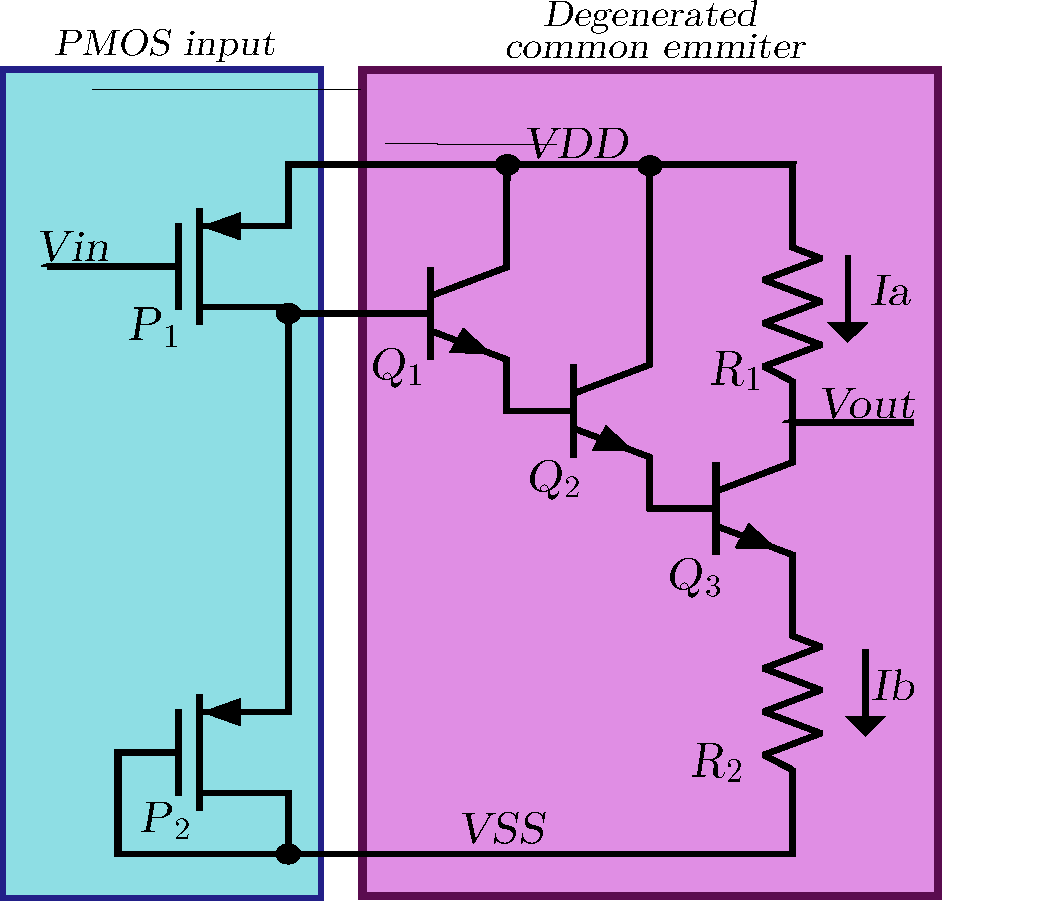
\includegraphics[width=0.5\textwidth]{audio002.pdf}
        \caption{audio002 amplifier schematic.}
        \label{audio002}
\end{figure}

\subsection{Circuit explanation}
This amplifier uses again a PMOS input in order to increase the input impedance of the amplifier. In order to increase the gain, a triple Darlington arrangement is used in order to increase the gain current and to improve temperature variations in comparison to a standard Darlington arrangement.

In this amplifier, in order to better define the initial operating point, the PMOS input stage is composed of two PMOS transistors: a current source PMOS ($P_2$) with its gate connected to $V_{SS}$, and an input PMOS with its gate connected to $V_{IN}$. This configuration ensures that the DC operating point is established through the relationship between the bias current of $P_2$ and the bias current of the base of $Q_1$.  

Since $P_2$ operates in saturation, the variation in current caused by a $\Delta V_{in}$ is primarily directed to the base of $Q_1$, so its essential to increase the $L$ of $P_{2}$ in order to reduce the channel modulation effect.

 A degeneration is putted  at the emitter of $Q_3$ in order to make the gain relation more linear. The trade off is that the gain is smaller then a non-degenerated system.

 The output impedance of the system is $R_1 || (R_{0Q3}+R_2)$

 In order to find the output transcondutance of the system, first the current gain of $P_1$ must be expressed.
 To better find the transcondutance its important to understand the equivalent emitter resistance in comparison to the driving signal. The emitter resistance can be broth up to the base by multiplying its value by $\beta$. Meaning in a small signal equivalent circuit, the equivalent resistance can be expressed approximately as $R_2 \times \beta_{Q1} \times \beta_{Q2} \times \beta_{Q3}$. Since the source of $P_2$ is connected to the node that varies with the total NPN current, the total transcondutance of the system can be expressed as
 
 \begin{equation}
     g_{mP1} (1 - g_{mbP2} \times R_2 \times \beta_{Q1} \times \beta_{Q2} \times \beta_{Q3} ) .
 \end{equation}
Meaning the amplifier as a gain expressed as

\begin{equation}
    A_v \approx          \beta_{Q1} \times \beta_{Q2} \times \beta_{Q3} \times g_{mP1} (1 - g_{mbP2} \times R_2 \times \beta_{Q1} \times \beta_{Q2} \times \beta_{Q3}) \times R_1 || (R_{0Q3}+R_2)
\end{equation}

This is achieved by ignoring the the channel modulation effect of the MOS transistors and by ignoring other effects in the Bipolar transistors.

\end{document}
